\documentclass[12pt]{report}

% Packages
\usepackage[utf8]{inputenc}
\usepackage{graphicx}
\usepackage{geometry}
\geometry{margin=1in}
\usepackage{amsmath, amssymb}
\usepackage{hyperref}
\usepackage{float}
\usepackage{chngcntr}
\counterwithout{figure}{chapter}  


\makeatletter
\def\thickhrulefill{\leavevmode \leaders \hrule height 1pt\hfill \kern \z@}
\def\maketitle{
    \thispagestyle{empty}
    \begin{center}
        \vskip 4pt
        {\Large American University of Armenia \par}
        \vskip -7pt
        \rule{13cm}{0.05em} \par
        {\large Zaven and Sonia Akian College of Science and Engineering \par}
    \end{center}
    \vfill
    \begin{center}
        {\Huge \textbf{Light Up puzzle as an Artificial Intelligence Problem: Analysis and Evaluation} \par}
        \vspace{5mm}
        {\Large CS246 / CS346 Project Report \par}
        \vfill
        {\Large Anna Gasparyan, Ani Baghumyan, Izabella Atajanyan \par}
        \vspace{3mm}
        {\Large Instructor: Monika Stepanyan \par}
    \end{center}
    \vfill
    \begin{center}
        {\large Summer 2026 \par}
    \end{center}
    \cleardoublepage
}
\makeatother

\begin{document}

\maketitle

\begin{center}
    {\LARGE \textbf{Abstract}}
\end{center}
\vspace{5mm}

Light Up, also known as Akari is a Japanese puzzle game with challenging solutions but rather simple rules. It requires placing light bulbs on a grid with black and white cells until the whole grid is lit up, while following a set of constraining rules, making it an interesting problem for studying different algorithmic approaches.

In this project, we are going to treat Light Up as a computational problem rather than just a puzzle, and explore and compare multiple algorithmic approaches. The goal is not only to solve it efficiently, but also to understand how different methods try to solve the problem under the same conditions. This includes examining how they handle constraints, how they reduce the search space, and how their performance changes depending on puzzle difficulty, size and other factors.

The project focuses on modeling Light Up puzzle in a way that allows the application of different algorithms, including systematic search, constraint-based reasoning, and optimization techniques. The results are analyzed based on performance, efficiency, and scalability. By comparing these approaches, the project aims to understand strengths and limitations of each algorithm, and to provide a clearer understanding of how each of them can be applied to the same problem.


\vspace{2mm}
\textbf{Keywords:}  light up, akari, constraint satisfaction, local search, hill climbing, backtracking, simulated annealing, SAT, CSP, DFS


\newpage

\tableofcontents
\listoffigures
\newpage

\chapter{Introduction}
\section{Background of the Light Up puzzle}
\indent 

Light Up is a binary determination puzzle published by \textbf{Nikoli}\cite{nikoli}, which is a Japanese publisher focused on logical games and puzzles. As of 2011, three full books consisting of only Light Up puzzles have been published by this publisher. The puzzle is not merely a curiosity: deciding whether a Light Up instance has a solution is NP-complete, shown by McPhail\cite{mcphail} through a reduction from Circuit-SAT. Solving time therefore grows exponentially in the worst case, and no algorithm removes that limit; what a better algorithm can do is push it further away, which is what this project sets out to measure. 



\section{Rules}

The rules of the game are rather simple. Light Up is played on a rectangular board of black and white cells; all the instances used in this project are square, of size $N \times N$. The player places light bulbs in white cells. A bulb sends rays of light horizontally and  vertically, illuminating its entire row and column unless the light is blocked by a black cell. No two bulbs may shine on each other, meaning no two bulbs should be on the same row or column, unless blocked from each other by a black cell.  Black cells might have numbers written on them (from 0 up to 4), which indicate the number of bulbs that should be placed adjacent to them. Two cells are considered adjacent if they share a common edge. Blank black cells might have any number of bulbs adjacent to them. The player solves the puzzle, if they manage to light up all the white cells while following all the rules(Figure \ref{fig:example}). 

\begin{figure} [H]
    \centering
    \includegraphics[width=0.6\linewidth]{59ED429E-C5DC-474F-BA71-9CEB906A913D.jpg}
    \caption{7 × 7 Light Up puzzle instance before and after solving}
    \label{fig:example}
\end{figure}



\chapter{Literature Review}

This literature review evaluates some approaches that have been used for solving the Light Up puzzle, including backtracking, constraint propagation, local search, and satisfiability.

\indent

\section{Hill Climbing and Simulated Annealing}

Libo Sun, James Browning, Roberto Perera in their paper "Shedding some light on light up with artificial intelligence" \cite{light_up_ai} solved the puzzle using an approach involving heuristic search. The authors tested \textit{Hill Climbing} and \textit{Simulated Annealing} using a fitness function that measured the percentage of lit cells while penalizing "conflicts", such as bulbs shining on each other or incorrect numbers of bulbs around black cells. 

To formalize the problem, the board was represented as a two-dimensional array of single digits, each representing a particular value: \textit{0} for black cells with 0, \textit{1} for black cells with 1, \textit{2} for black cells with 2, \textit{3} for black cells with 3, \textit{4} for black cells with 4, \textit{5} for blank black cells, \textit{6} for empty white cells, \textit{7} for cells with a bulb inside them, \textit{8} for cells that are lit up by a bulb, \textit{9} for cells that cannot have bulbs adjacent to them(Figure \ref{fig:boardarray}).
\begin{figure}[H]
    \centering
    \includegraphics[width=0.4\linewidth]{Screenshot 2026-07-23 at 16.15.38.png}
    \caption{Example of board representation as a numerical array\cite{light_up_ai}}
    \label{fig:boardarray}
\end{figure}


At the initial state, the light bulbs would be placed randomly. The available actions are adding a bulb, removing a bulb, moving a bulb from one cell to another empty cell. 
The authors firstly implemented a plain hill climbing that focuses on immediate improvement. For each step, the algorithm generates a set of neighboring states by applying one of the available actions. Secondly, the initialization was optimized before the implementation of hill climbing. Some cells may only have unique way for placing bulbs in, thus the searching space can be reduced, so initialization was optimized. They compared a \textbf{2-action model} (add or remove a bulb) against a \textbf{3-action model} (add, remove, or \textbf{move} a bulb to a different cell). The algorithm selects the neighbor with the highest fitness value. If no neighbor is better than the current state, it terminates, which frequently leads to getting stuck in \textbf{local maxima}. 

To overcome the local maxima problem inherent in Hill Climbing, the authors used Simulated Annealing, which achieved \textbf{100\% accuracy} across all 30 unique test cases. Unlike Hill Climbing, if a randomly selected move is worse than the current state, the algorithm may still accept it based on a probability function. This probability depends on a "temperature" that starts high (allowing many bad moves to escape local maxima) and gradually decreases over time. As \textit{T} approaches zero, the algorithm behaves more like a standard hill climber, eventually settling into a \textbf{global maximum} (the solution). The inclusion of the "move" action in the 3-action model was specifically cited as a reason for significantly higher accuracies in this algorithm. 

It was concluded that simulated annealing had the best performance, while the hill climbing with optimized initialization had the second best and the vanilla hill climbing was the worst.

\section{SAT and Backtracking}

In his "Analysis of Akari" paper\cite{analysis_akari} Bram Pulles approached the puzzle by developing SAT and Backtracking solver systems. Before developing the solvers, the author executed a trivial solver, which was used for preprocessing that identified certain placements where the number of available spaces around a black cell exactly matches its numerical clue. It also identifies the cells where a bulb cannot be placed due to existing lights or clues with number zero on them(Figure \ref{fig:trivial}).  

\begin{figure}[H]
    \centering
    \includegraphics[width=1\linewidth]{Screenshot 2026-07-28 at 16.48.10.png}
    \caption{Examples of trivial solutions\cite{analysis_akari}}
    \label{fig:trivial}
\end{figure}

For effective solving, Pulles implemented a SAT solver that uses the Z3 theorem prover by translating the entire board into a boolean formula. This formula is based by three primary conditions: every numbered cell must have the correct amount of adjacent bulbs, every white cell must be illuminated at least once, and no two bulbs can be positioned in a row or column without a wall between them.  By converting the puzzle into a satisfiability problem, the system can solve complex 40x40 puzzles in less than a second, although it may slow down on nearly empty boards that lack sufficient constraints. 

Finally, the author implemented a backtracking solver using depth-first search that begins with base solution from the trivial solver, then sorts the rest of the candidates such that the candidates adjacent to numbered cells are prioritized, because satisfying the number constraints is the difficult part. The solver recursively explores placements while checking for instances where a numerical clue cannot be met to trigger early backtracking and avoid wasted computation. 

The performance results show a massive speed difference between the two approaches. On standard puzzles, the SAT solver is much faster because it uses the highly optimized Z3 library, allowing it to solve large 40 × 40 boards in less than a second. In contrast, the backtracking solver can take several minutes to solve even a small 14 × 14 puzzle. However, there is one interesting exception: when a board is almost completely empty with very few walls, the SAT solver slows down significantly. In these specific cases, the simpler backtracking approach actually finishes the job faster.

\section{Relation to our work}

Light Up has also been treated explicitly as a constraint problem. Çelik et al.\cite{celik2009} model Akari alongside three other grid puzzles in both Answer Set Programming and Constraint Programming, and compare the two formalisms on representation and on running time. That work is concerned with comparing declarative formalisms, rather than with the behaviour of a search procedure, which is what we set out to measure.

Taken together these strands shape our own design. Pulles is the closest precedent for what we build, although he does not describe it in the vocabulary of constraint satisfaction: his trivial solver is constraint propagation, his ordering of candidates so that cells beside numbered walls come first is a variable-ordering heuristic, and his early check for a clue that can no longer be satisfied is the same test our forward-checking solver performs. His inference, however, runs once as preprocessing. Our contribution is to state the puzzle as a CSP, move that inference inside the search loop so that it runs to a fixpoint at every node, and then measure what the change is worth. Where Pulles delegates the search itself to the Z3 library, we implement every solver ourselves, which is what makes a comparison of search behaviour meaningful. We also reimplement the hill climbing and simulated annealing of Sun et al., so that the ordering they report between the two can be tested on instances other than their own.


\chapter{Solution approaches}

\section{CSP}
\label{sec:csp}
The first approach to solving the Light Up puzzle is to formulate it as a Constraint Satisfaction(CSP) problem. A CSP is defined by a set of variables X, a domain of possible values D, and a set of constraints C:

\bigskip
X = \{all white cells on the board\}
\newline 

D = \{bulb, empty\}
\newline

        C = \{C1, C2, C3\}
\bigskip

C1: No two bulbs illuminate each other

C2: Every white cell is illuminated by at least one bulb

C3: Every numbered black cell has exactly the specified number of adjacent bulbs
\bigskip

Consider some definitions to express constraints formally. Let $\text{\textbf{\textit{sight}}}(w)$ be the set of white cells that share its row or column with a white cell $w \in X$ and are not separated from it by a black cell. For a numbered black cell, let $n_c$ denote its clue value and $N_c$ the set of white cells orthogonally adjacent to it. Let $b_w \in \{0, 1\}$ indicate whether a cell has a bulb or not. Finally, let $\text{\textbf{\textit{Clues}}}$ denote the set of numbered black cells on the board.
\newline
Using this notation, the three constraints can be written formally as:
\newline
  
  \(C_1: \quad \forall\, w \in X,\ \forall\, w' \in \text{sight}(w): \quad b_w + b_{w'} \le 1\)
\newline

\(C_2: \quad \forall\, w \in X:           \quad b_w + \sum_{w' \in \text{sight}(w)} b_{w'} \ge 1\)

\bigskip

  \(C_3: \quad \forall\, c \in \text{Clues}: \quad \sum_{x \in N_c} b_x = n_c\)
  
\bigskip
Solving the problem means finding an assignment of values from D to every variable in X that satisfies all the constraints in C. The three constraint families are all \emph{counting} constraints, in that each bounds how many bulbs a region may contain: at least one over a cell's line of sight, at most one over a wall-free segment, and exactly $n_c$ over a clue's neighbours. The standard techniques we apply to them, backtracking search with forward checking and with constraint propagation, follow Russell and Norvig\cite{aima}. Three backtracking approaches are implemented, all are formed based on the same problem formulation, but differ in how much reasoning they do before and during branching: a naive baseline, backtracking with forward checking, and a full inference. Comparing these three approaches would mean measuring the effect of inference on the search process.

\subsection{Naive Backtracking}

  The naive solver visits the white cells in a fixed row-major order and, at each one,
  first tries placing a bulb and only falls back to leaving it empty if that fails. Each
  attempt is followed by a consistency check; if it passes, the search recurses to the
  next cell in order, and if it fails, the attempt is undone before the next value is
  tried. This is a plain depth-first search over the CSP defined in Section~\ref{sec:csp},
  with no variable-ordering heuristic (cells come strictly in reading order, however
  unpromising) and no value-ordering heuristic beyond always preferring a bulb first.

  Consistency is checked by fully re-evaluating the board from scratch at every node
  rather than by maintaining any state across nodes: the partial assignment is validated
  against $C_1$ and $C_3$, and the set of currently lit cells is recomputed from nothing
  each time. On top of this, one further rule is required for the search to be usable at
  all rather than merely correct, the \emph{doomed-cell} rule: once an unlit cell $w$ and
  every cell in $\text{sight}(w)$ have all been decided empty, $w$ can never be lit again,
  so $C_2$ has become unsatisfiable and the branch is abandoned immediately rather than
  only being caught by the goal test many nodes later. Without this rule the
  search would remain complete, since every full assignment is still checked at the
  leaves, but it would exhaustively wander through enormous, obviously dead subtrees even
  on tiny boards.

  A complete assignment is only accepted once every white cell has been decided and a
  final goal test confirms all three constraints hold, including the exact clue counts
  required by $C_3$. Because nothing is propagated ahead of time and nothing is reused
  between nodes, this solver's cost grows with the number of nodes it visits, which is
  what the smarter variants below are built to reduce.


\subsection{Backtracking with Forward Checking}

  The forward-checking and full-inference solvers share the same underlying search
  procedure and differ only in how much they infer at each node; this subsection
  describes what they share, and the next two describe how each configures that shared
  inference step.

  Unlike the naive solver, both maintain explicit state across the whole search instead of
  rescanning the board: each white cell's status (bulb, empty, or still undecided), a live
  count of how many bulbs currently light each cell, and a trail recording the order
  assignments were made in, so that backtracking can undo exactly what changed instead of
  rebuilding everything. Board geometry -- which cells each cell can see, and which cells
  are adjacent to each clue -- is computed once before the search starts, rather than
  being recomputed on every check.

  Placing a bulb immediately forward-checks $C_1$: every cell in its line of sight is
  marked empty the moment the bulb is placed, since a bulb in any of those cells would now
  conflict with it. If one of those cells already holds a bulb, this is detected as an
  immediate conflict rather than being discovered later by a broader check. Both solvers
  also share the same variable-ordering heuristic when enabled: prefer an undecided
  neighbor of whichever unfinished clue has the least slack (the fewest free neighbors
  relative to how many bulbs it still needs), and once every clue is settled, prefer a
  candidate lighter of whichever unlit cell has the fewest remaining cells that could
  light it. This is the standard most-constrained-variable heuristic, adapted to Light
  Up's counting constraints rather than a fixed arity. Value ordering still tries a bulb
  before leaving a cell empty, since a bulb makes concrete progress toward $C_2$ and lets
  the checks below fail faster if the choice turns out to be wrong.

  Where the two solvers actually differ is the lookahead performed before each recursive
  call. The forward-checking configuration performs a check-only pass: it does not modify
  any assignment, it only decides whether the current partial assignment can still
  possibly lead to a solution, using two conditions. The first is a clue window check for
  $C_3$: writing $\text{placed}(c)$ and $\text{free}(c)$ for the number of a clue's
  neighbors that are currently bulbs or still undecided respectively, the branch fails the
  moment $\text{placed}(c) > n_c$ or $\text{placed}(c) + \text{free}(c) < n_c$ for any
  clue $c$. The second is a support check for $C_2$: an unlit cell that is already decided
  empty, with no undecided cell left in its own position or line of sight, has lost every
  remaining chance of ever being lit, and the branch fails immediately rather than only at
  the final goal test. Neither condition assigns a value on its own -- they only answer
  whether the branch is still alive -- which is why this configuration is described as
  pruning rather than full inference.


\subsection{Backtracking with Full Inference}

  The full-inference configuration keeps everything described above, but replaces the
  prune-only lookahead with a step that actively assigns values it can prove are forced,
  repeating until a full pass makes no further changes -- i.e., until a fixpoint is
  reached. Three rules drive this:

  \begin{align}
  \text{placed}(c) = n_c &\;\Longrightarrow\; \forall x \in \text{free}(c):\ b_x \leftarrow 0
  &&\text{(saturated clue)} \\
  \text{placed}(c) + |\text{free}(c)| = n_c &\;\Longrightarrow\; \forall x \in \text{free}(c):\ b_x \leftarrow 1
  &&\text{(exhausted clue)} \\
  \bigl|\{x \in \{w\} \cup \text{sight}(w) : x \text{ undecided}\}\bigr| = 1,\ w \text{ unlit}
  &\;\Longrightarrow\; b_x \leftarrow 1 &&\text{(forced lighter)}
  \end{align}

  A saturated clue has already received exactly as many bulbs as its number requires, so
  every remaining undecided neighbor must be empty or $C_3$ would be violated. An
  exhausted clue is the mirror case: so few undecided neighbors remain that all of them
  must hold a bulb, or the clue could never reach its required count. A forced lighter
  covers $C_2$ directly: once an unlit cell has exactly one remaining cell able to light
  it, that cell must be a bulb, or the cell would go permanently unlit. Applying one rule
  can create the conditions for another -- a forced bulb, for instance, may itself
  saturate a different clue -- so all three are re-checked in a loop until nothing changes
  in a full pass.

  Because this configuration assigns values rather than only pruning, a meaningfully
  larger share of the puzzle in this solver is resolved by logic instead of by branching,
  which is tracked separately as propagations rather than search nodes when comparing
  solvers in Chapter~\ref{chap:results}. This inference step is also run once before the
  very first branching decision is made, so purely deductive consequences of the puzzle's
  initial clues -- a clue of 0 forcing all of its neighbors empty, or a clue of 4 forcing
  all of them to hold a bulb -- are resolved before the search ever branches at all.


\section{Local search}

Local search was used for the second solution approach. Two solvers were implemented: hill climbing and simulated annealing. Both solvers are implemented as incomplete algorithms that operate on a complete-state formulation, meaning they evaluate entire board configurations unlike the CSP approach. 

Both solvers share several specific components. They navigate the search space using a 3-action model: adding a bulb, removing a bulb, and moving one bulb from one cell to another available cell. 

To ensure efficiency both solvers share an infrastructure that begins by precalculating entire board's geometry. Before starting the search, the program determines which white cells can see each other across the board's rows and columns. This allows the agent to immediately know which cells are illuminated every time a move is made instead of scanning the board every time. This significantly speeds up the evaluation of each state during the search.

The search starts using an informed initialization strategy, which provides a more structured starting point than a pure random assignment. The system follows a process where it chooses random unlit cells and places bulbs one by one until every white square on the board is illuminated. This approach also guarantees that no two bulbs look at each other at the beginning of the search, which is a big advantage. This results in a high quality starting configuration that ensures that the entire board is lit, even though some numerical clues might be violated.

The progress to the solution is measured by a cost function that the agent works to minimize. The function acts as a scoring system where the solution has a cost of zero and each violation increases the score. The agent is penalized for every white cell that remains unlit, for every instance where a numbered black cell has the wrong number of adjacent bulbs, and when there are bulbs shining on each other:

\[\ C(s) = \sum (Unlit White Cells)+\sum_ {c  \in  Clues}| n_c - a_c| +\sum (Bulb Collisions),\]
where for every numbered black cell \textit{c}, $n_c$ is the required number of bulbs and $a_c$ is  the actual number of adjacent bulbs. With informed initialization, search initially starts with zero bulb collisions.

\subsection{Hill Climbing}

This implementation utilizes a steepest-ascent logic combined with a "greedy" neighbor selection process. In each step, the algorithm samples 30 random neighbors from the current state using the 3-action model. The agent only transitions to a neighbor if it strictly improves the fitness (lowers the cost). If the best neighbor is not better than the current state, the agent identifies this as a local optimum. To escape these local optima, the solver immediately triggers a random restart, generating a completely new initial state and beginning the climb again until a solution is found or the timer expires. 

\subsection{Simulated Annealing}

The simulated annealing solver improves Hill Climbing by allowing the agent to occasionally accept moves that actually make the board state worse. This logic is designed to prevent the solver from getting stuck in a local dead end where no single move looks like an improvement, but a solution still exists in a different part of the search space. On each step, the agent proposes exactly one random change using the 3-action model. If this change lowers the cost function, it is always accepted immediately. However, if the change increases the cost, the solver calculates a probability based on a "temperature" value to decide whether to take the move anyway.  As the search goes on, this temperature gradually drops, which makes the agent selective about accepting bad moves. On early stages, when the temperature is high, the agent very frequently jumps to different configurations to explore the board. As the temperature drops, it becomes much stricter, eventually settling into a final arrangement and becoming more like regular hill climbing. If the temperature falls below a minimum threshold without a solution being found, the solver performs a "reheat". This resets the temperature to the starting high point and generates a completely new board configuration, allowing the search to begin again until a perfect arrangement is discovered.

\section{Experimental setup}
\label{sec:setup}

Comparing five solvers requires a supply of instances, so we wrote a
generator that constructs puzzles solution-first. It places walls at a
requested density, mirrored through the board centre for the symmetry that
published puzzles conventionally have, and then builds a valid bulb
placement by repeatedly putting a bulb on a randomly chosen cell that is
still unlit. A cell that is unlit lies outside the line of sight of every
bulb already placed, so this can never create a conflict, and the procedure
terminates with the whole board illuminated. Every wall then receives, with
some probability, the number of bulbs the placement happens to put beside
it, and finally the bulbs are removed. What remains is a puzzle that is
solvable by construction, since the placement we started from is a
solution. It is not necessarily uniquely solvable, and we return to that
point in Chapter~\ref{chap:results}.

Three difficulty presets control the two densities: easy boards are 25\%
walls with every wall numbered, medium 18\% and 80\%, and hard 12\% and
55\%. The names describe the effort a human solver would expend, since
sparse clues make the chain of deductions longer.

We evaluated five board sizes ($7\times7$, $10\times10$, $14\times14$,
$18\times18$ and $25\times25$) against the three presets, with five seeded
instances in each combination, giving 75 distinct puzzles. Every solver
received exactly the same 75 puzzles, and each run was given a budget of
five seconds, for 375 runs in total. Because the generator is a
deterministic function of the board size, the preset and the seed, and
because the two randomised solvers take the instance seed as their own,
every measurement can be reproduced exactly from those three values; the
instances themselves need not be stored.

For every run we record whether it succeeded, the wall-clock time, the
number of search nodes (or, for local search, the number of candidate
states evaluated), the number of conflicts, and the number of assignments
made by propagation rather than by branching. Local-search runs also record
the lowest cost reached, which measures how close a failed run came to a
solution. A run counts as successful only when the validator confirms that
the returned placement satisfies $C_1$, $C_2$ and $C_3$. We deliberately do
not compare against a stored answer, because a puzzle may admit several
valid solutions and any of them is a correct result.


\chapter{Evaluation}
\label{chap:results}

\section{Results}

Table~\ref{tab:solvesize} reports how many instances each solver finished
within the budget, broken down by board size. The ordering is unambiguous.
Full inference solved every instance we generated; forward checking failed
only on the largest boards; the naive baseline degraded from perfect at
$7\times7$ to nothing at all at $25\times25$. Among the local-search
solvers, simulated annealing matched the naive baseline overall while hill
climbing solved barely more than a quarter of the set.

\begin{table}[H]
  \centering
  \begin{tabular}{lcccccc}
    \hline
    solver & $7\times7$ & $10\times10$ & $14\times14$ & $18\times18$ & $25\times25$ & total \\
    \hline
    naive backtracking & 15/15 & 14/15 & 11/15 & 5/15 & 0/15 & \textbf{45/75} \\
    forward checking & 15/15 & 15/15 & 15/15 & 14/15 & 9/15 & \textbf{68/75} \\
    full inference & 15/15 & 15/15 & 15/15 & 15/15 & 15/15 & \textbf{75/75} \\
    hill climbing & 14/15 & 5/15 & 2/15 & 0/15 & 0/15 & \textbf{21/75} \\
    simulated annealing & 15/15 & 15/15 & 11/15 & 4/15 & 0/15 & \textbf{45/75} \\
    \hline
  \end{tabular}
  \caption{Instances solved within the five-second budget, by solver and
  board size (15 instances per cell, 75 in total).}
  \label{tab:solvesize}
\end{table}

\subsection{The effect of inference}

Figure~\ref{fig:scaling} shows how sharply the three backtracking variants
diverge. Measured in search nodes, the gap between the naive solver and
the informed ones widens with board size: roughly sevenfold at
$7\times7$, fortyfold at $10\times10$ and a hundred and sixtyfold at
$14\times14$. Inference therefore does not merely subtract a constant
amount of work, it changes how the cost grows.

The clearest single measurement concerns the published $7\times7$ instance
of Pulles~\cite{analysis_akari}. The naive solver needs 308 search nodes to
solve it and forward checking needs 12, while full inference needs
\emph{none at all}: 41 propagation steps derive the whole solution without
a single branching decision. This is consistent with how such puzzles are
made, since a published puzzle is designed to be solvable by human
deduction, and our propagation rules are a mechanical form of exactly that
deduction. It is worth noting that the effect is much rarer on our own
instances, where only 3 of 15 boards at $7\times7$ and none beyond
$14\times14$ were solved without any search. We suspect the reason is that
our generator guarantees solvability but not uniqueness, so its boards are
less tightly constrained and correspondingly less deducible.

\begin{figure}[H]
    \centering
    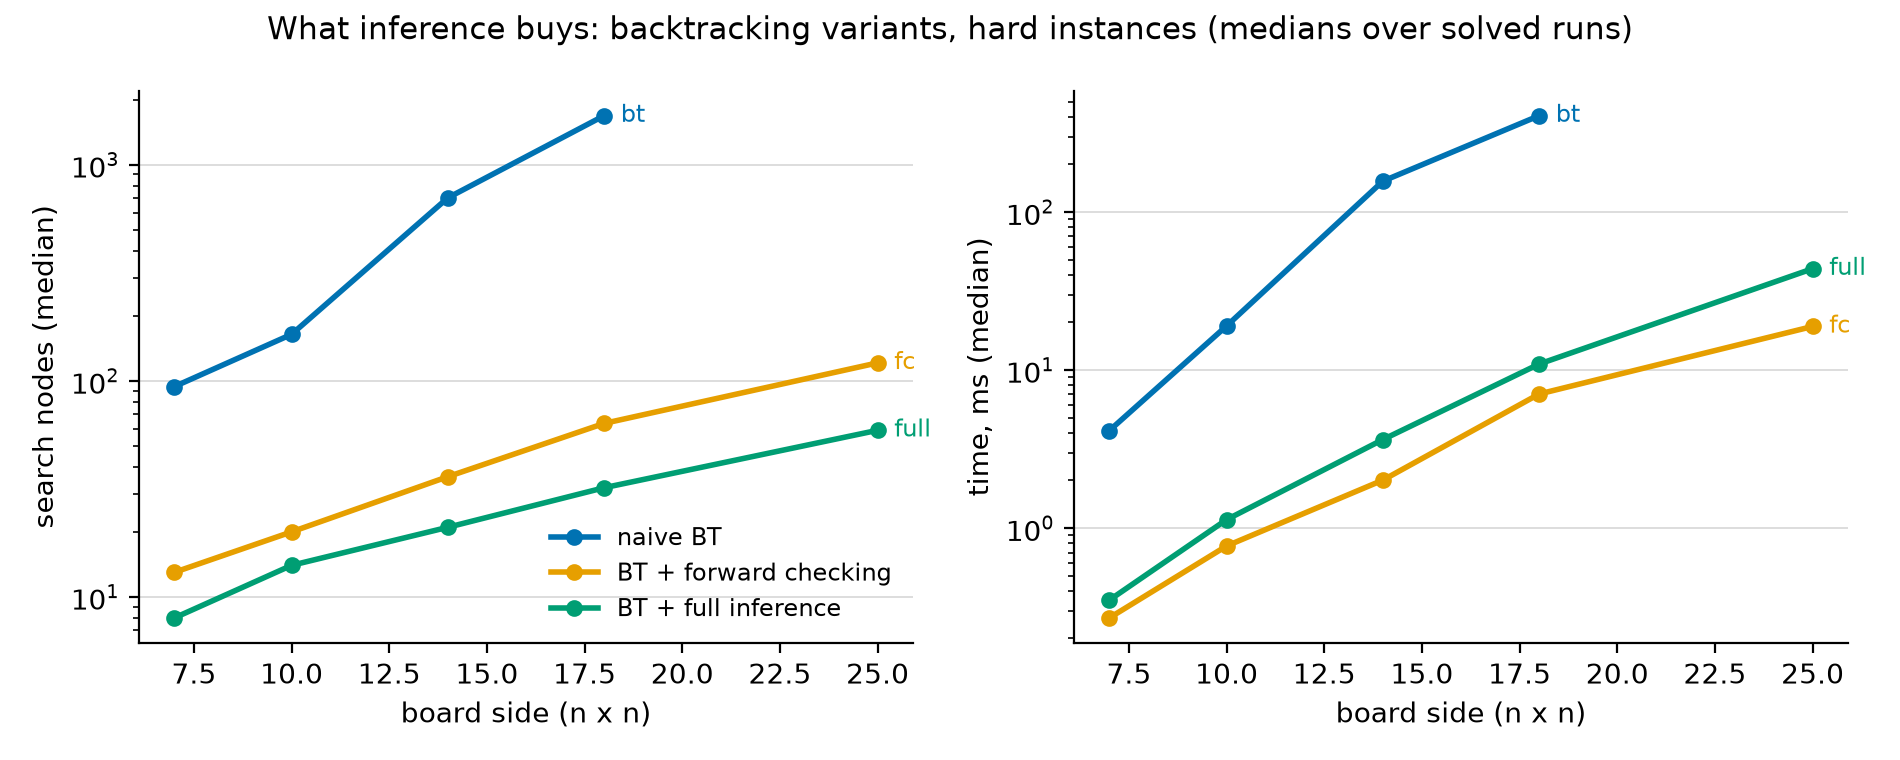
\includegraphics[width=\linewidth]{fig1_bt_scaling.png}
    \caption{Median search nodes and median solving time against board
    size for the three backtracking variants, on hard instances. Medians
    are taken over solved runs only; the naive curve stops at $18\times18$
    because it solved nothing beyond that.}
    \label{fig:scaling}
\end{figure}

One qualification matters here, because the obvious summary of
Figure~\ref{fig:scaling} is misleading. Full inference always expands
about half as many nodes as forward checking, but fewer nodes do not
automatically mean less time: propagation is an investment paid at every
node, and whether it pays back depends on how much there is to deduce.
Table~\ref{tab:fcfull} separates the two solvers by clue density. On
clue-dense (easy) boards full inference wins at every size, by a factor of
thirty-five at $25\times25$; on sparse (hard) boards, where propagation
usually finds nothing, forward checking is consistently the faster of the
two. Figure~\ref{fig:scaling} plots hard instances and therefore shows the
side of this trade favourable to forward checking. Full inference is
nevertheless the more reliable solver, since it is the only one that never
exceeded the budget.

\begin{table}[H]
  \centering
  \begin{tabular}{llccccc}
    \hline
    preset & solver & $7\times7$ & $10\times10$ & $14\times14$ & $18\times18$ & $25\times25$ \\
    \hline
    easy & forward checking & 0.40 & 0.69 & 2.80 & 9.42 & 275.42 \\
     & full inference & 0.31 & 0.61 & 1.11 & 3.88 & 7.73 \\
    medium & forward checking & 0.35 & 1.06 & 6.07 & 150.54 & 18.11 \\
     & full inference & 0.35 & 0.79 & 2.53 & 6.77 & 20.57 \\
    hard & forward checking & 0.27 & 0.77 & 2.01 & 7.05 & 18.87 \\
     & full inference & 0.35 & 1.13 & 3.63 & 10.91 & 43.78 \\
    \hline
  \end{tabular}
  \caption{Median solving time in milliseconds for the two informed
  backtracking solvers, split by difficulty preset. Whether propagation
  pays for itself depends on clue density rather than on board size.}
  \label{tab:fcfull}
\end{table}

\subsection{Complete search against local search}

Figure~\ref{fig:paradigms} compares all five solvers on hard instances.
Simulated annealing outperformed hill climbing at every size, solving 19
of 25 hard instances against 11, and 45 of all 75 against 21. This
reproduces, on instances of our own, the central result reported by Sun,
Browning and Perera~\cite{light_up_ai}, and it does so with an independent
implementation.

The manner of failure is as informative as the counts. Because our cost
function reports how many violations remain, a failed run still tells us
how close it came. Hill climbing ended its failed runs a median of 13
violations short of a solution, simulated annealing only 5.5, and in one
twenty-second run on a hard $14\times14$ board hill climbing restarted
12{,}496 times while never resolving a single remaining violation. This is
a local optimum in its purest form: every single move available made the
board worse, so a solver that accepts only improvements could not move at
all. Simulated annealing escapes precisely because it will accept a worse
state temporarily.

\begin{figure}[H]
    \centering
    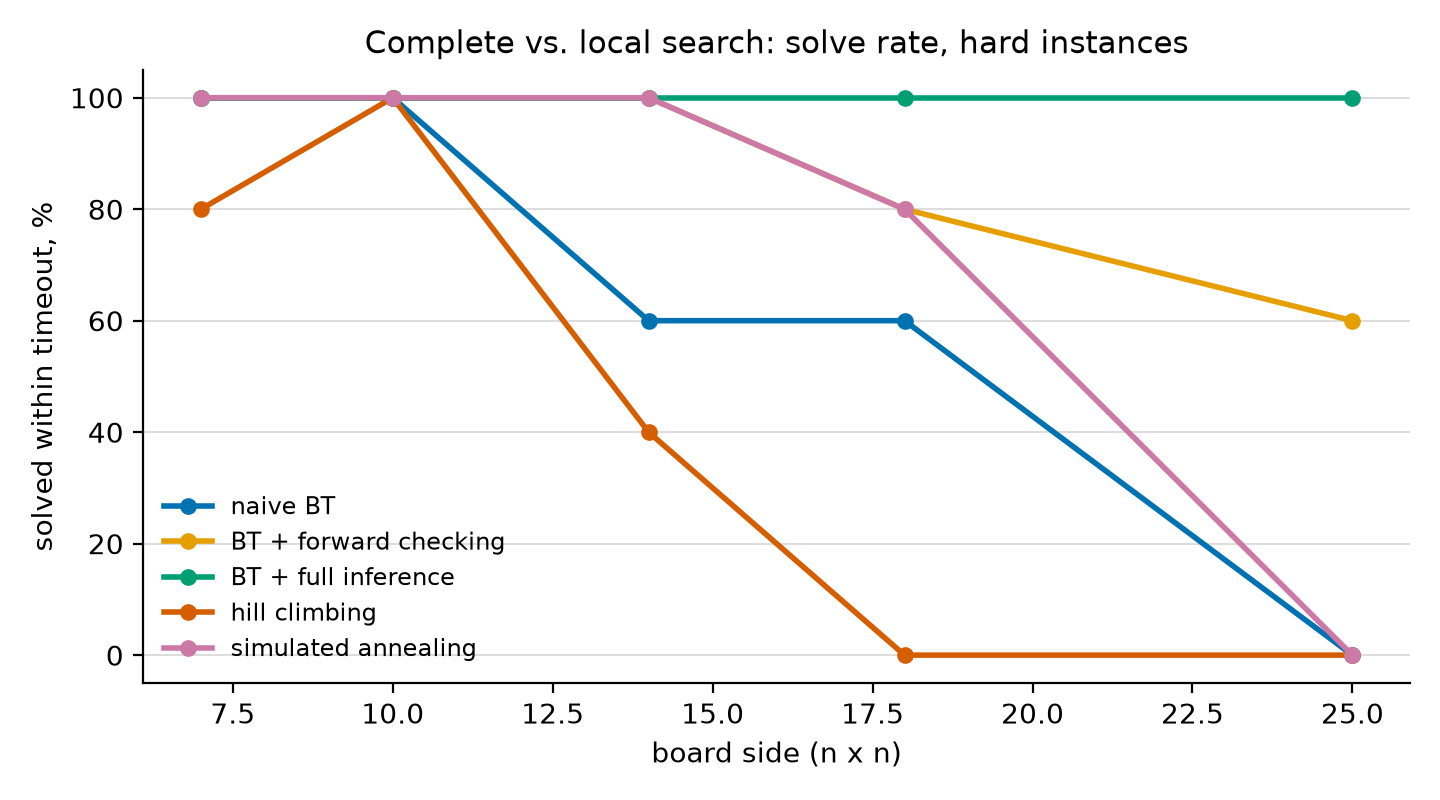
\includegraphics[width=0.85\linewidth]{fig2_paradigms.png}
    \caption{Percentage of hard instances solved within the budget, by
    board size, for all five solvers.}
    \label{fig:paradigms}
\end{figure}

Two limitations of local search should be stated plainly. Neither solver
can ever prove that a board has no solution, since both only ever report
that they have not found one; and within the budget we used, complete
search with inference outperformed both of them at every size we tested.

\subsection{What makes an instance hard}

Our difficulty presets vary the density of walls and clues, and we
expected denser boards to be easier for every solver. Figure~\ref{fig:difficulty}
shows that this is not what happens. Hill climbing solved none of the easy
or medium instances at $14\times14$ yet solved some of the hard ones, and
at $10\times10$ the pattern is starker still: nothing on easy or medium,
and all five hard instances. Simulated annealing behaves the same way,
solving 19 of 25 hard instances but only 13 of 25 easy ones. The informed
backtracking solvers show the opposite preference, forward checking
solving all 25 easy instances and 22 hard ones.

\begin{figure}[H]
    \centering
    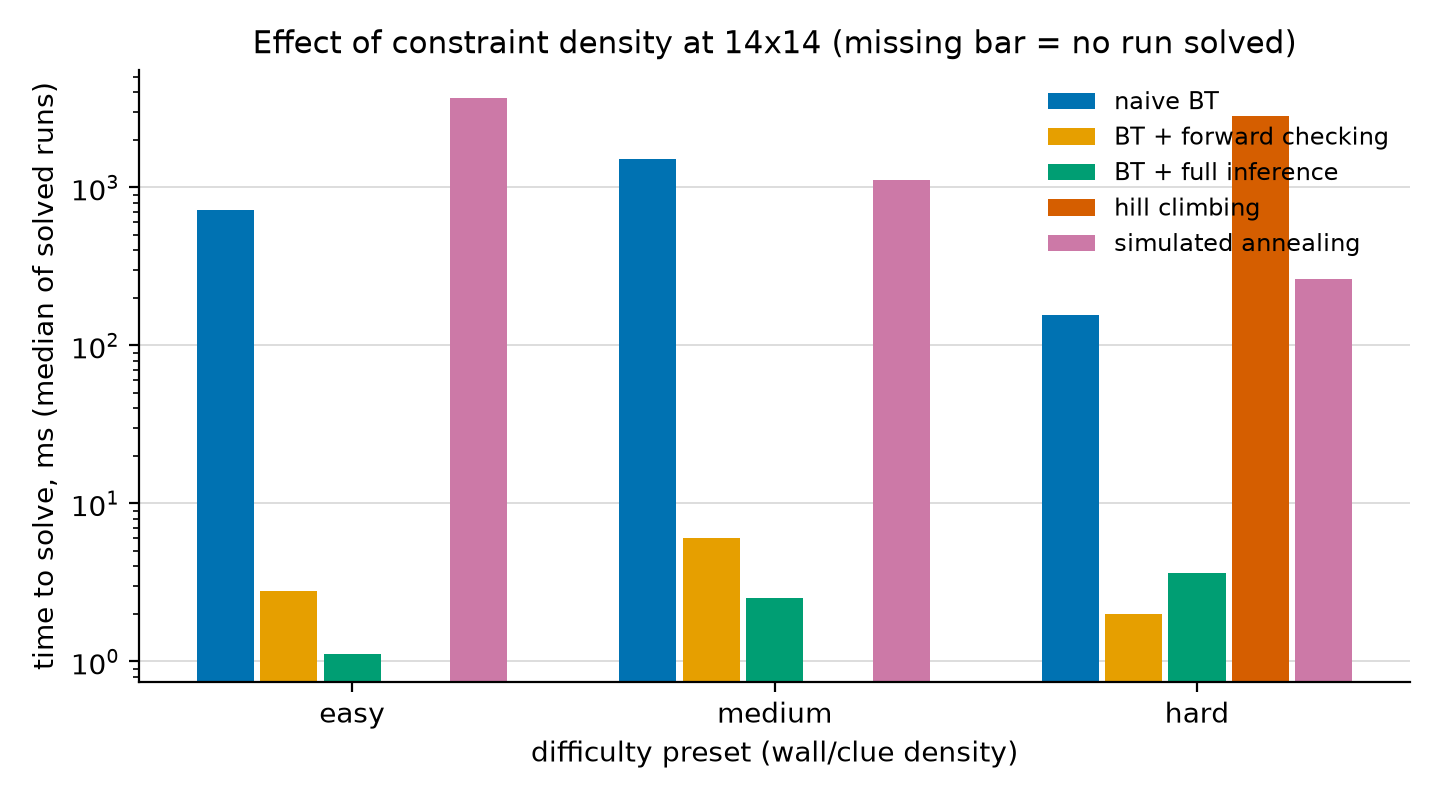
\includegraphics[width=0.85\linewidth]{fig3_difficulty.png}
    \caption{Median solving time by difficulty preset at $14\times14$. A
    missing bar means that no run of that solver was solved within the
    budget.}
    \label{fig:difficulty}
\end{figure}

The explanation is that a clue means different things to different
solvers. To a solver that reasons about constraints, a clue is
information: it is what the propagation rules of
Section~\ref{sec:csp} consume, so more clues make the board easier. To a
local-search solver, which can only evaluate a complete assignment, each
clue is one more penalty term in the cost function; dense boards therefore
have a more rugged landscape with more local optima, and are harder. Note
that the raw search space moves in the opposite direction, since our hard
preset leaves about 172 white cells at $14\times14$ against about 146 for
easy, so this cannot be explained by problem size. Our presets predict the
difficulty a human would experience, which depends on the length of the
deduction chain, and not the difficulty a solver experiences.

\subsection{Sensitivity to the time budget}

Because a five-second budget is an arbitrary choice, we repeated the whole
sweep with ten seconds on the identical instances. Almost nothing changed:
the naive solver gained three instances, forward checking and simulated
annealing two each, full inference none, and hill climbing exactly none
(Figure~\ref{fig:budget}). No instance was lost, which also confirms that
the runs are properly seeded and deterministic. Doubling the budget helps a
solver that is merely slow, and does nothing for a solver that is stuck, so
the differences reported above are structural rather than artefacts of the
budget we chose.

\begin{figure}[H]
    \centering
    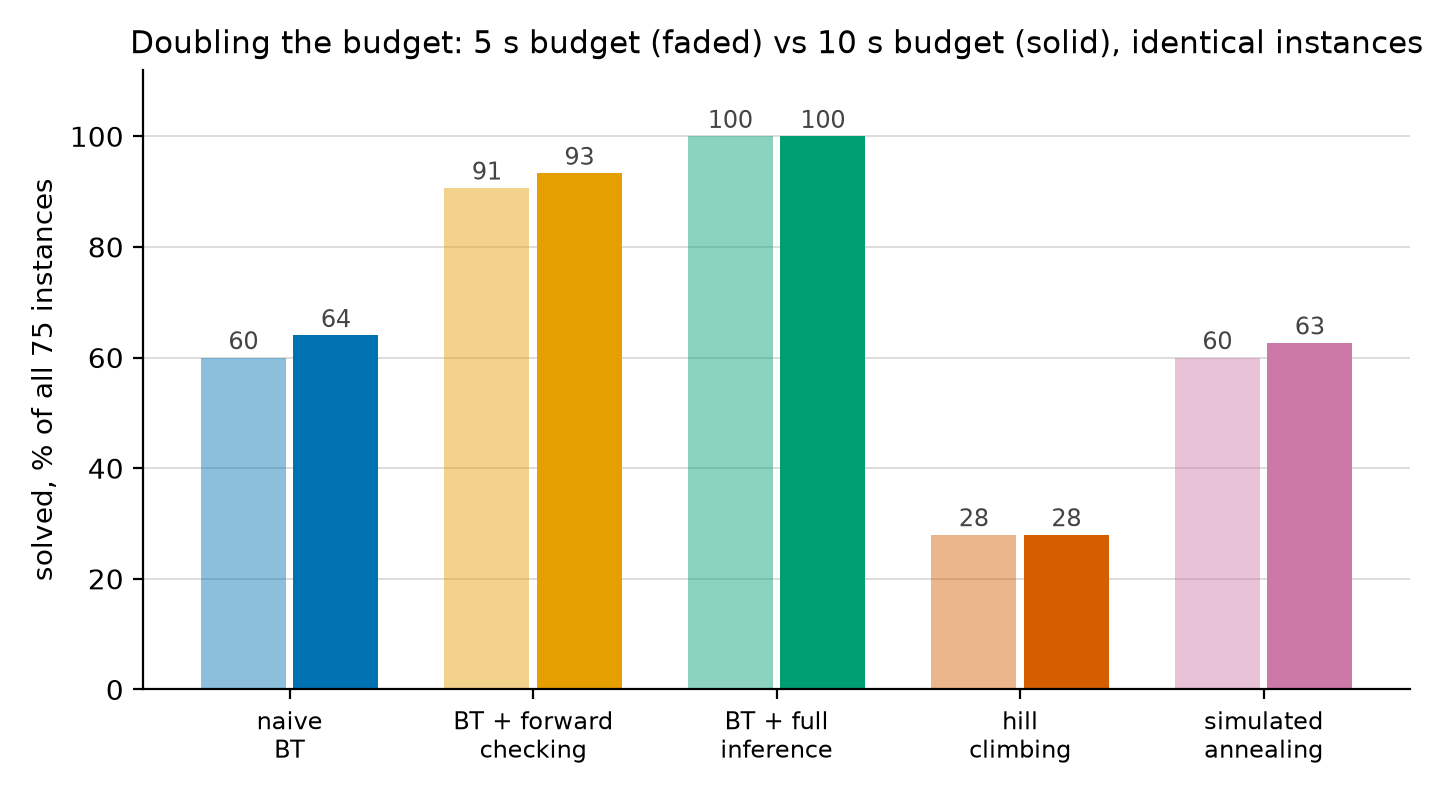
\includegraphics[width=0.85\linewidth]{fig4_budget.png}
    \caption{Instances solved under a five-second and a ten-second budget
    on identical instances, for each solver.}
    \label{fig:budget}
\end{figure}

\subsection{Limitations}

Three caveats apply to the numbers above. We used five instances per
combination of size and difficulty, which is enough to support the
aggregate comparisons but means that a single instance moves a per-cell
rate by twenty points, so the individual cells of Table~\ref{tab:solvesize}
should be read as indicative. All medians are taken over solved runs only,
which introduces a survivorship effect: the naive solver's median node
count falls between $14\times14$ and $18\times18$ not because it improved
but because only the easiest instances at the larger size contributed to
the median, so solve rate and search effort must always be read together.
Finally, all timings are wall-clock measurements from a single machine
running CPython, so the comparisons between solvers are meaningful while
the absolute milliseconds are not.

\section{Conclusion}

We set out to compare several ways of solving the same problem under
identical conditions, and the comparison produced a clear ordering.
Inference dominates: adding propagation to backtracking turned a solver
that failed on two thirds of the largest boards into one that solved every
instance we generated, and on a published puzzle it removed the need to
search at all. The gain grows with board size, which means inference
changes the growth rate of the cost rather than merely reducing it.

The comparison also produced three results we did not anticipate. Fewer
search nodes do not automatically mean less time, because propagation must
be paid for at every node and only repays that cost when the board carries
enough clues to deduce from. Simulated annealing beat hill climbing by a
wide margin, confirming published work, and the way hill climbing failed —
stalling one violation away from a solution across twelve thousand
restarts — illustrates the local-optimum problem more concretely than any
description of it could. Most surprisingly, sparse boards proved easier for
our solvers than dense ones, which tells us that the density presets we
built model human difficulty rather than search difficulty.

Finally, doubling the time budget changed almost nothing, which is the
result that gives us most confidence in the rest: the differences we
measured come from how the solvers are built, not from how long they were
allowed to run.

\section{Possible Future work}

Three directions follow directly from the limitations above. Our generator
guarantees that a puzzle is solvable but not that its solution is unique,
and adding the uniqueness filter described by Pulles~\cite{analysis_akari}
would let us test our suspicion that uniquely solvable boards are
substantially more deducible. A second direction is a satisfiability
formulation: our propagation rules are already a form of unit propagation,
so writing our own conjunctive normal form encoding and DPLL solver would
let us compare a clause-based formulation against the constraint-based one
directly, without relying on an external solver as previous work has done.
Third, since our difficulty presets turned out to predict human rather
than machine difficulty, they could be recalibrated against measured
search effort, which would also give a principled way to generate
instances of a target hardness.


\begin{thebibliography}{9}

\bibitem{analysis_akari}
Pulles, B., "Analysis of Akari", Radboud University, Jan. 9, 2021, \href{https://www.cs.ru.nl/bachelors-theses/2021/Bram_Pulles___1015194___Analysis_of_Akari.pdf}{https://www.cs.ru.nl/bachelors-theses/2021/Bram\_Pulles\_\_\_1015194\_\_\_Analysis\_of\_Akari.pdf}

\bibitem{light_up_ai}
Sun, L., Browning, J., Perera, R., "Shedding some light on light up with artificial
intelligence", Auburn University, Jul. 23, 2021, \href{https://arxiv.org/pdf/2107.10429}{https://arxiv.org/pdf/2107.10429}

\bibitem{mcphail}
McPhail, B., "Light Up is NP-complete", 2005, \href{https://www.researchgate.net/publication/249927572_Light_Up_is_NP-complete}{https://www.researchgate.net/publication/249927572\_Light\_Up\_is\_NP-complete}

\bibitem{aima}
Russell, S., Norvig, P., \emph{Artificial Intelligence: A Modern Approach}, 4th ed., Pearson, 2021.

\bibitem{nikoli}
Nikoli, "Light Up (Bijutsukan)", \href{https://www.nikoli.co.jp/en/puzzles/akari/}{https://www.nikoli.co.jp/en/puzzles/akari/}

\bibitem{celik2009}
Çelik, M., Erdoğan, H., Tahaoğlu, F. H., Uras, T., Erdem, E., "Comparing ASP and CP on Four Grid Puzzles", 16th RCRA International Workshop (RCRA 2009), Reggio Emilia, Italy, CEUR-WS Vol. 589, \href{https://ceur-ws.org/Vol-589/paper01.pdf}{https://ceur-ws.org/Vol-589/paper01.pdf}


\end{thebibliography}

\end{document}

